\documentclass[dvips]{article}
\usepackage{amsmath}
\usepackage{amsfonts}
\usepackage{amssymb}
\usepackage{amsthm}
\usepackage{authblk}
\usepackage[italian]{babel}
\usepackage[utf8]{inputenc}
\usepackage{flafter}
\usepackage{float}
\usepackage[T1]{fontenc}
\usepackage{graphics}
\usepackage{placeins}
\usepackage{listings}
\usepackage{graphicx}
\usepackage{enumerate}
\usepackage{booktabs}
\usepackage{caption}
\usepackage{pstricks,pstricks-add,pst-math,pst-xkey}
\usepackage{listings}
\lstloadlanguages{Java}
\usepackage{ifthen}
\usepackage{multicol}
\usepackage[scriptsize]{caption}
\usepackage{verbatim}
\usepackage{hyperref}
\usepackage{eurosym}
\usepackage{pythonhighlight}
\usepackage{pdfpages}
\usepackage{enumitem}
\usepackage{siunitx}
\usepackage{tabularx}
\usepackage{relsize}
\usepackage{calculator}
\usepackage[margin=1.6in]{geometry}

\begin{document}

\title{Moti in campi elettrici e magnetici}
\author{Giovanni Durante}
\affil{Liceo Scientifico M. Grigoletti\\
classe 4 C opzione scienze applicate\\
 a.s. 2020-21}
\date{27 marzo 2021}

%titolo autore scuola
\begin{titlepage}
	\maketitle
\end{titlepage}

%indice qui o in fondo
\tableofcontents
 
\section{Abstract}
Lo scopo di questo paper è investigare i moti di particelle cariche in presenta di campi elettrici e magnetici per poi ricavare le traiettorie percorse da suddette particelle, eventualmente dotate di velocità iniziale. Sono stati analizzati casi particolari in cui i vettori campo giacciono in posizioni specifiche, questo non ha effetti sull'analisi in quanto è la posizione reciproca dei vettori che determina il tipo di moto risultante. Sono stati classificati 3 generi di moti: moto uniformemente accelerato, moto elicodale, moto cicloidale. 

\section{Introduzione}
Una particella carica, dotata o meno di velocità iniziale, segue diverse traiettorie in presenza di campi elettrici e magnetici a seconda di come questi sono posizionati. Sia il campo magnetico che quello elettrico impartiscono una accelerazione alla particella carica, tuttavia mentre la forza di Lorentz sviluppa una accelerazione normale alla velocità che tende a formare un moto circolare uniforme, la forza data dal campo elettrico è in grado di modificare la direzione e l'intensità della velocità iniziale. In seguito sarà fornità una analisi di tutti questi fenomeni ed anche delle applicazioni reali che sfruttano questi moti per accelerare le particelle. Tratterò il sincrociclotrone utilizzando la fisica relativistica poiché, avendo le particelle massa molto piccola, anche una minima accelerazione può raggiungere velocità comparabili a quella della luce. Studierò ogni caso utilizzando cariche positive.

\section{Contenuti}
\subsection{Primo caso}
La velocità, la forza generata dal campo elettrico e il campo magnetico hanno stessa direzione, verso. \newline
Ottengo che la forza magnetica è nulla $F_m = vqBsin(0) = 0$ e che la particella è accelerata grazie al campo elettrico $F_e = qE,  \quad a_m = \dfrac{qE}{m}$. Quindi come legge oraria si ha: 
\begin{equation}
    x(t) = vt + \dfrac{1}{2}\dfrac{qEt^2}{m}
\end{equation}

\subsection{Secondo caso}
Campo magnetico ed elettrico hanno stessa direzione, la velocità è normale a questi (in questo caso $\Vec{E}$ e $\Vec{B}$ coincido con l'asse X).
\begin{figure}[H]
    \centering
    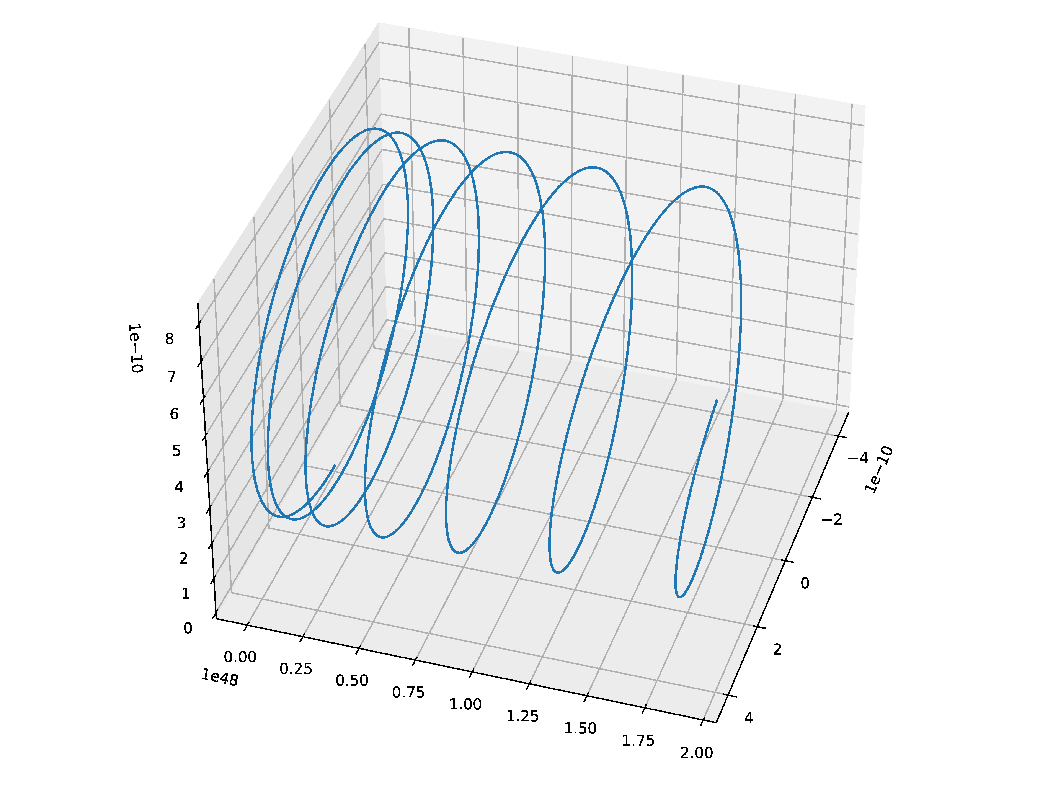
\includegraphics[width=9cm]{elica.eps}
\end{figure}
La forza di Lorentz agisce deviando in ogni istante la direzione della velocità, agisce come forza centripeta: $F_m = qvB = \dfrac{mv^2}{r}$, la velocità non cambia intensità. Si tratta di un moto circolare uniforme che avviene sul piano $ax=0$ \footnote{Il piano Y-Z}.
La forza del campo elettrico imprime una accelerazione costante alla particella nella direzione dell'asse X, si tratta quindi di moto elicoidale accelerato, dove la accelerazione dal campo elettrico è $a_x = \dfrac{Eq}{m}$.  Per le componenti y e z si tratta di moto armonico (la proiezione della particella che si muove di moto circolare uniforme su i 2 assi): $y(t)=Rsin(qBt)$ e $z(t) = R(1- cos(qBt))$. Dove $R$ è il raggio della circonferenza che si ricava dalla equazione della forza centripeta: $R = \dfrac{mv}{qB}$. Ottengo infine
\begin{equation}
    \begin{cases}
      y(t) = Rsin(qBt)\\ 
      x(t)= \dfrac{1}{2}at^2+v_{\parallel}t\\
      z(t) = R (1 - cos(qBt))
    \end{cases}
\end{equation}

\subsection{Terzo caso}
Velocità iniziale nulla, $\Vec{B} \perp \Vec{E}$,  $\Vec{E}$ è rivolto verso l'asse Y, $\Vec{B}$ verso l'asse Z.
La particella inizialmente accelera verso l'asse Y, si genera quindi la forza di Lorentz perpendicolare alla velocità, la traiettoria della particella devia verso l'ascissa positivo. La forza risultante che descrive questo è $\Vec{F} = q(\Vec{E}+\Vec{v}\times\Vec{B})$. Non si presenta alcun moto verso l'asse Z poiché nessuna forza agisce verso questo asse.
Sviluppando:  
\[m\Vec{a} = qE\Vec{j} + q(\Vec{v}\times\Vec{B}) = qE\Vec{j} + q
\begin{vmatrix}
\Vec{i} & \Vec{j} & \Vec{k}\\
v_x & v_y & 0\\
0 & 0 & B
\end{vmatrix} = qE\Vec{j} + qv_yB\Vec{i} -qv_xB\Vec{j}
\]
Posso esprimere la accelerazione come la derivata della velocità e scomporla nelle sue componenti: $m\dfrac{dv_x}{dt}\Vec{i} = (qv_yB)\Vec{i}$ e $m\dfrac{dv_y}{dt}\Vec{j} = (qE - qv_xB)\Vec{j}$.
Per ottenere le due velocità da queste equazioni è necessario risolvere una equazione differenziale, ho utilizzato Sympy, una libreria Python per il calcolo simbolico \footnote{Per passare dalla soluzione generica, che ha 2 paramentri ignoti, alla soluzione esatta ho fornito a Sympy l'informazione che $v_y(0) = 0$ }. Le due velocità sono quindi:
\[
v_y = \dfrac{E}{B}sin(\dfrac{qBt}{m}) \quad v_x = \dfrac{E}{B}(1-cos(\dfrac{qBt}{m}))
\]
Considerando che la velocità è la derivata dello spazio sul tempo, si può ricavare la traiettoria della particella facendo l'integrale di queste due funzioni ottenendo quindi:

\begin{equation}
    \begin{cases}
      y(t) = \dfrac{E}{B}(1-cos(\dfrac{qBt}{m}))\\
      x(t) = \dfrac{E}{B}(t-\dfrac{msin(\tfrac{qBt}{m})}{qB})\\
      z(t) = 0
    \end{cases}
\end{equation}
Si tratta di un cicloide.

%%  qui immagine che non si piazza bene...
\begin{figure}[h!]
    \begin{center}
    %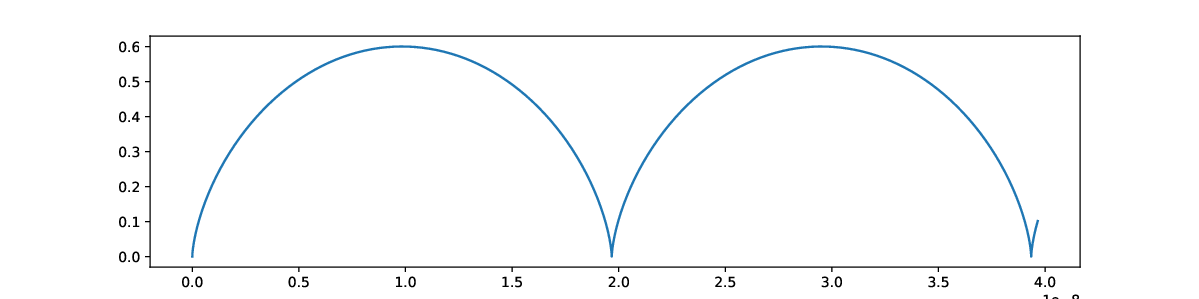
\includegraphics[width=13cm]{cicloide.eps}
    \end{center}
\end{figure}



\subsection{Applicazioni}
\subsubsection{Ciclotrone}
Il ciclotrone (e le sue evoluzioni) sfruttano i campi elettrici e magnetici per accelerare particelle cariche.
\begin{figure}[H]
    \centering
    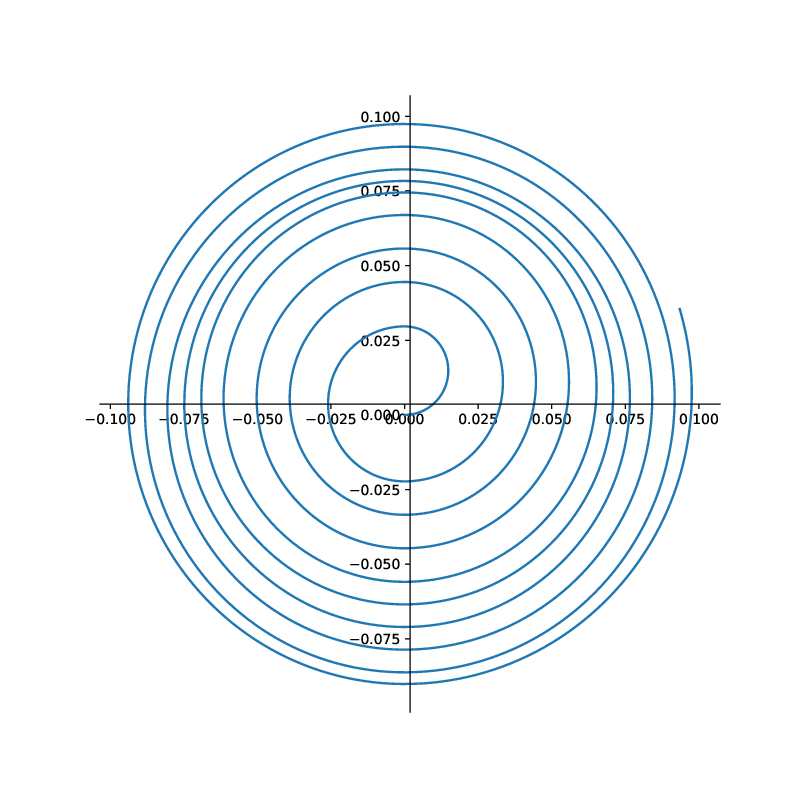
\includegraphics[width=7cm]{ciclotrone.eps}
\end{figure}
Il ciclotrone è composto da 2 elettrodi a D separati da una intercapedine, tutto questo in uno spazio attraversato da un campo magnetico uscente. La particella è introdotta perpendicorlarmente al campo magnetico nell'intercapedine, a questo punto la particella è soggetta alla forza del campo elettrico e accelera secondo $a = \dfrac{qE}{m}$. Intato la forza di Lorentz agisce come forza centripeta (si instaura un moto circolare). Quando la particella penetra una delle D non è più soggetta alla accelerazione da campo elettrico poiché questo è nullo all'interno di un conduttore carico isolato, la velocità è ora costante. Quando la particella esce dalla D (seguendo sempre una traiettoria circolare) la polarità delle D si inverte, la particella accelera nuovamente per poi rientrare nella D. Ad ogni iterazione di questo ciclo la particella accelera sempre di più ed il raggio della circonferenza aumenta poiché $R = \dfrac{mv}{qB}$ dove $m, q, B$ sono costanti. 
\subsubsection{Simulazione della traiettoria del ciclotrone}
\begin{python}
import numpy as np
import matplotlib.pyplot as plt

# calcola la forza risultante
def ftot(p,v,t): 
    f = np.zeros(3)
    """se la particella si trova nel mezzo delle due D
    allora calcola la accelerazione data dal campo elettrico, 
    altrimenti considera la accelerazione centripeta."""
    if np.abs(p[0]) < dist/2:
        f[0] = E*q*np.cos(w*t)
    else:
        f = q*np.cross(v,B)
    return f


def trajectory(dt):
    p = np.array([[0,0,0]])
    v = np.array([[0,0,0]])
    t = np.array([0])
    i = 0
    """finché la particella è dentro il raggio del ciclotrone calcola
    istante per istante (dt) la forza risultante, la velocità istanea
    (che incrementa ad ogni passaggio attraverso la intercapedine) e la 
    posizione della particella (che varia in base alla velocità). Tutti 
    questi dati sono salvati negli array così posso conoscere la velocità 
    finale, il tempo totale impiegato e la posizione di uscita"""
    while np.linalg.norm(p[i]) < radius:
        t = np.append(t, t[i]+dt)
        f = ftot(p[i], v[i], t[i])
        v = np.vstack((v, (v[i] + f / m * dt)))
        p = np.vstack((p, (p[i] + v[i+1] * dt))) 
        i+=1
    return p[:i], v[:i], t[:i]


q, m, dist, radius = 1.6e-19, 1.67e-27, 90e-6, 0.1
V=50000
B = np.array([0.0,1.5,0.0])

# poiché le D sono un un condensatore piano il campo elettrico è questo
E = V/dist
w = q*np.linalg.norm(B)/m
p,v,t = trajectory(5e-12)

fig, ax = plt.subplots(figsize=(13,13))
ax.spines['left'].set_position('center')
ax.spines['bottom'].set_position('center')
ax.spines['right'].set_color('none')
ax.spines['top'].set_color('none')
ax.xaxis.set_ticks_position('bottom')
ax.yaxis.set_ticks_position('left')
# il moto avviene sul piano X-Z quini seleziono tutti gli elementi di p[0] e p[2]
plt.plot(p[:,0], p[:,2])
\end{python}

\subsubsection{Sincrociclotrone}
Il ciclotrone non è in grado di accelerare particelle a velocità prossime a quelle della luce poiché non considera gli effetti relativistici delle velocità. Il Sincrociclotrone risolve queste limitazioni considerando l'aumentare della massa con la velocità. Infatti la velocità angolare è data da:
\[
\omega = \dfrac{qB}{\gamma m}
\]
dove $\gamma = \dfrac{1}{\sqrt{1-\tfrac{v^2}{c^2}}}$. Questo permette al circuito che inverte la polarità di attivarsi in fase con l'uscita della particella dalla D secondo $T = \dfrac{1}{f} = \dfrac{2\pi \gamma m}{qB}$. Risultando quindi in una maggiore efficienza.

\section{Conclusione}
Non tutte le parti del mio lavoro potevano essere conclusi con gli strumenti matematici di cui disponevo. Ho raggirato il problema utilizzando un software CAS (neanche troppo sofisticato) arrivando ad una conclusione ragionevole. È evidente, purtroppo, come dal punto di vista metodologico questo sia scorretto. 

\end{document}


